% -*- mode : latex; coding: utf-8 -*-
\chapter{Background and Related Work}
\label{sec:backgrounds}

\section{ARM Cortex-M4 Architecture}

The STM32F446 implements ARM Cortex-M4F with 180MHz operation and 8-region MPU capability. Key features include:

\textbf{Performance}: 225 DMIPS with Harvard architecture enabling simultaneous instruction fetch and data access. Single-cycle multiply and hardware divide instructions optimize automotive control algorithms.

\textbf{Debug Capabilities}: Data Watchpoint and Trace (DWT) unit provides cycle-accurate performance monitoring. The DWT\_CYCCNT register enables precise timing measurement down to 5.56 nanoseconds.

\section{Memory Protection Unit}

The MPU provides hardware-enforced memory access control with:
\begin{itemize}
    \item 8 simultaneous memory regions with independent configuration
    \item Minimum 32-byte regions with power-of-2 sizing
    \item Read/write/execute permission combinations
    \item Hardware validation operating parallel with memory operations
\end{itemize}

\begin{figure}[h]
\centering
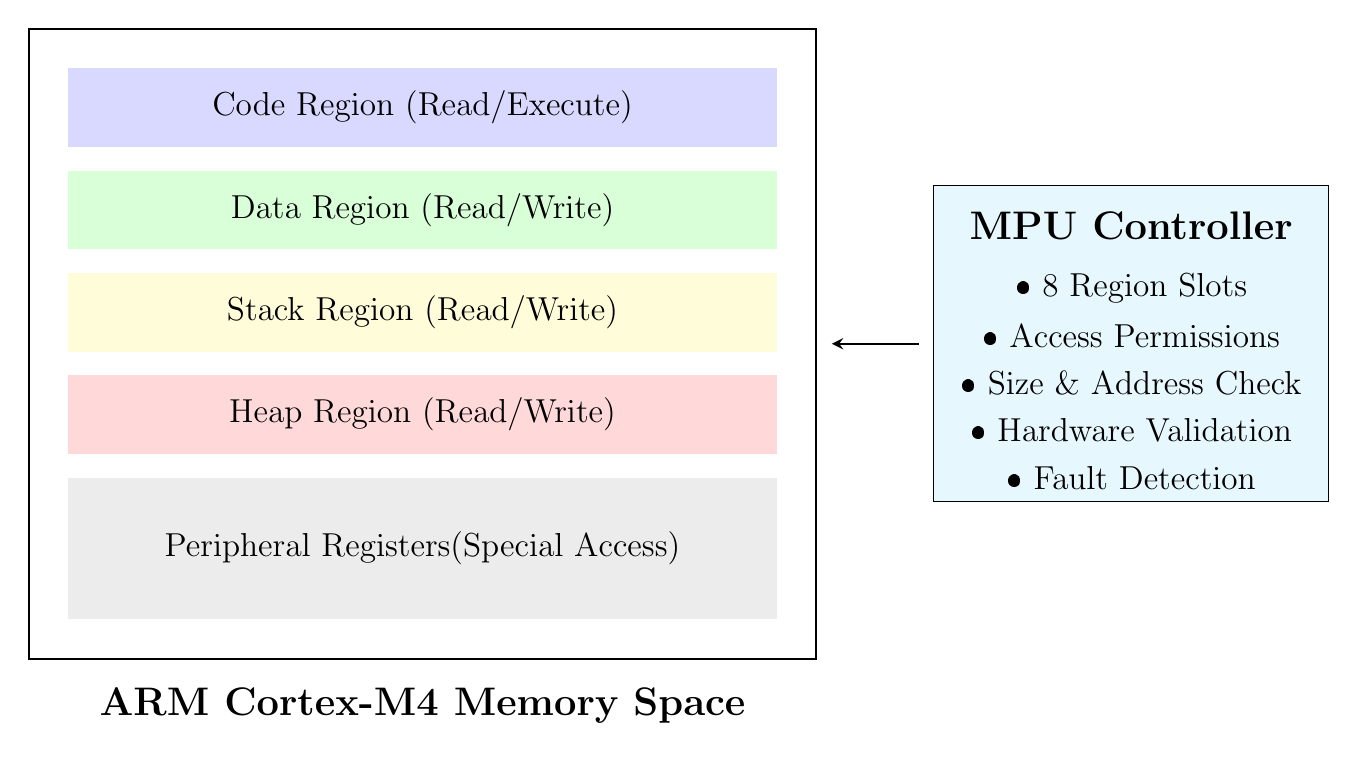
\begin{tikzpicture}[scale=1.0]
    % Memory layout - larger and more spaced
    \draw[thick] (0,0) rectangle (10,8);
    \node at (5,-0.6) {\Large\textbf{ARM Cortex-M4 Memory Space}};

    % Memory regions with better spacing
    \fill[blue!15] (0.5,6.5) rectangle (9.5,7.5);
    \node at (5,7) {\large Code Region (Read/Execute)};

    \fill[green!15] (0.5,5.2) rectangle (9.5,6.2);
    \node at (5,5.7) {\large Data Region (Read/Write)};

    \fill[yellow!15] (0.5,3.9) rectangle (9.5,4.9);
    \node at (5,4.4) {\large Stack Region (Read/Write)};

    \fill[red!15] (0.5,2.6) rectangle (9.5,3.6);
    \node at (5,3.1) {\large Heap Region (Read/Write)};

    \fill[gray!15] (0.5,0.5) rectangle (9.5,2.3);
    \node at (5,1.4) {\large Peripheral Registers\\(Special Access)};

    % MPU controller box with better positioning
    \draw[thick] (11.5,2) rectangle (16.5,6);
    \fill[cyan!10] (11.5,2) rectangle (16.5,6);
    \node at (14,5.5) {\Large\textbf{MPU Controller}};

    % MPU features with proper spacing
    \node at (14,4.7) {\large • 8 Region Slots};
    \node at (14,4.1) {\large • Access Permissions};
    \node at (14,3.5) {\large • Size \& Address Check};
    \node at (14,2.9) {\large • Hardware Validation};
    \node at (14,2.3) {\large • Fault Detection};

    % Connection arrow with better positioning
    \draw[thick,->,>=stealth] (11.3,4) -- (10.2,4);
\end{tikzpicture}
\caption{ARM Cortex-M4 MPU Memory Protection Architecture}
\label{fig:mpu_architecture}
\end{figure}

Dynamic reconfiguration during context switches enables task isolation but introduces overhead requiring characterization for real-time applications.

\section{Automotive Requirements}

\textbf{Real-time Constraints}: Engine control requires sub-millisecond response (1-5ms periods), chassis systems need <10ms for safety interventions, body electronics operate at 50-100ms.

\textbf{ISO 26262 Standards}: ASIL C/D systems require hardware-based memory protection for fault isolation. Higher levels mandate ≥90\% diagnostic coverage, making MPU violation detection valuable.

\textbf{Security}: Connected vehicles require attack surface mitigation and code integrity protection against injection attacks.

\section{Related Work}

Previous embedded system security work lacks automotive-specific performance analysis. The Tock OS project demonstrates hardware MPU combined with Rust language safety, providing insights for automotive three-tier trust models where safety-critical functions, comfort features, and applications coexist with appropriate isolation.